\documentclass[a4paper]{article}
\usepackage{graphicx}
\usepackage{coqdoc}
\usepackage{amsmath}
\usepackage{amssymb}
\usepackage[all]{xy}
\usepackage{mathpartir}
\usepackage{tabto,calc}
\usepackage{onecolceurws}

\newcommand{\tto}{\twoheadrightarrow}
\newcommand{\flavio}[1]{{\color{red}#1}}

\newcommand{\comm}[1]{\tabto{\CurrentLineWidth}\fbox{\begin{minipage}[t]{0.98\linewidth-\TabPrevPos} #1 \end{minipage}}}

\newtheorem{theorem}{Theorem}[section]
\newtheorem{definition}{Definition}[section]
\newtheorem{lemma}{Lemma}[section]

\title{A Formalization of the (Compositional) Z Property}

\author{
Flávio L. C. de Moura and Leandro O. Rezende\\ Dept. de Ciência da Computação\\
                Universidade de Brasília \\ flaviomoura@unb.br
}

\institution{}




\begin{document}
\maketitle

\begin{abstract}
  Rewriting theory is a well established model of computation
  equivalent to the Turing machines, and the most well known rewriting
  system is the $\lambda$-calculus. Confluence is an important and
  undecidable property related to the determinism of the computational
  process. Direct proofs of confluence are, in general, difficult to
  be done. Therefore, alternative characterizations of confluence can
  circumvent this difficulty for different contexts. This is the case
  of the so called Z property, which has been successfully used to
  prove confluence in several situations such as the
  $\lambda$-calculus with $\beta\eta$-reduction, extensions of the
  $\lambda$-calculus with explicit substitutions, the
  $\lambda\mu$-calculus, etc. In this work we present a direct and
  constructive proof that the Z property implies confluence.  In
  addition, we formalized our proof and an extension of the Z
  property, known as the Compositional Z, in the Coq proof assistant.
\end{abstract}
\vskip 32pt


\section{Introduction}

Confluence is an important and undecidable property concerning the
determinism of the computational process. In this sense, one says that
a program is confluent if every two ways of evaluating it, result in
the very same answer. In the particular case of Abstract Rewriting
Systems (ARS), which are the focus of this work, confluence can be
beautifully expressed by diagrams as we will see in the next section.

The contributions of this work are as follows:
\begin{itemize}
\item We present a new proof that the Z property implies confluence,
  which is direct and constructive.
\item The proof that the Z property implies confluence is formalized
  in the Coq proof assistant, and the presentation is made
  interleaving Coq code followed by an explanation in English of the
  code. In this way, the annotations are done directly in the Coq
  files using the coqdoc annotation style. We believe that this
  approach is interesting for those that are not familiar with the Coq
  proof assistant because the Coq code followed by English
  explanations gives a good idea on how they relate to each
  other. This discipline also forces a better organization of the
  formalization and of the proofs so that the explanation in English
  is comprehensible.
\item We formalize an extension of the Z property, known as
  compositional Z property, as presented in
  \cite{Nakazawa-Fujita2016}.
\end{itemize}

\section{The Z property implies Confluence}




  An ARS, say $(A,R)$, is defined as a pair composed of a set $A$ and
  binary relation over this set $R:A\times A$. Let $a,b\in A$. We
  write $a\to_R b$ (or $R\ a\ b$ in Coq) to denote that $(a,b)\in R$,
  and we say that $a$ $R$-reduces to $b$ in one step. The reflexive
  transitive closure of a relation \coqdocvar{R}, written as $\tto_R$, is
  defined by the following inference rules: \begin{mathpar}
  \inferrule*[Right={$(refl)$}]{~}{a \tto_R a} \and
  \inferrule*[Right={$(rtrans)$}]{a\to_R b \and b \tto_R c}{a \tto_R
  c} \end{mathpar} \noindent where $a,b$ and $c$ are universally
  quantified variables as one makes explicit in the corresponding Coq
  definition: \begin{coqdoccode}
\coqdocemptyline
\coqdocnoindent
\coqdockw{Inductive} \coqdocvar{refltrans} \{\coqdocvar{A}:\coqdockw{Type}\} (\coqdocvar{R}: \coqdocvar{Rel} \coqdocvar{A}) : \coqdocvar{A} \ensuremath{\rightarrow} \coqdocvar{A} \ensuremath{\rightarrow} \coqdockw{Prop} :=\coqdoceol
\coqdocnoindent
\ensuremath{|} \coqdocvar{refl}: \coqdockw{\ensuremath{\forall}} \coqdocvar{a}, (\coqdocvar{refltrans} \coqdocvar{R}) \coqdocvar{a} \coqdocvar{a}\coqdoceol
\coqdocnoindent
\ensuremath{|} \coqdocvar{rtrans}: \coqdockw{\ensuremath{\forall}} \coqdocvar{a} \coqdocvar{b} \coqdocvar{c}, \coqdocvar{R} \coqdocvar{a} \coqdocvar{b} \ensuremath{\rightarrow} \coqdocvar{refltrans} \coqdocvar{R} \coqdocvar{b} \coqdocvar{c} \ensuremath{\rightarrow} \coqdocvar{refltrans} \coqdocvar{R} \coqdocvar{a} \coqdocvar{c}.\coqdoceol
\coqdocemptyline
\end{coqdoccode}
The rules named (\coqdocvar{refl}) and (\coqdocvar{rtrans}) are called \textit{constructors}
in the Coq definition. The first constructor, namely \coqdocvar{refl}, states
the reflexivity axiom for $\tto_R$, while \coqdocvar{rtrans} extends the
reflexive transitive closure of \coqdocvar{R}, if one has at least a one-step
reduction. As a first example, let's have a look at the proof of
transitivity of $\tto_R$:


\begin{lemma} Let $\to_R$ be a binary relation over a set $A$. For
all $t, u, v \in A$, if $t \tto_R u$ and $u \tto_R v$ then $t \tto_R
v$.  \end{lemma}


 Despite its simplicity, the proof of this lemma will help us explain
the way in which we will relate English annotations with the proof
steps. Coq proofs are written between the reserved words \coqdockw{Proof} and
\coqdockw{Qed} (lines 1 and 9), and each proof command finishes with a
dot. Proofs can be structured with bullets (- in the first level, + in
the second level, * in the third level, ** in the fourth level, and so
on). The corresponding informal proof proceed as follows: The
corresponding lemma in Coq, named \coqdocvar{refltrans\_composition}, is stated
as follows: \begin{coqdoccode}
\coqdocemptyline
\coqdocnoindent
\coqdockw{Lemma} \coqdocvar{refltrans\_composition} \{\coqdocvar{A}\} (\coqdocvar{R}: \coqdocvar{Rel} \coqdocvar{A}): \coqdockw{\ensuremath{\forall}} \coqdocvar{t} \coqdocvar{u} \coqdocvar{v}, \coqdocvar{refltrans} \coqdocvar{R} \coqdocvar{t} \coqdocvar{u} \ensuremath{\rightarrow} \coqdocvar{refltrans} \coqdocvar{R} \coqdocvar{u} \coqdocvar{v} \ensuremath{\rightarrow} \coqdocvar{refltrans} \coqdocvar{R} \coqdocvar{t} \coqdocvar{v}.\coqdoceol
\coqdocnoindent
\coqdockw{Proof}.\coqdoceol
\coqdocindent{1.00em}
\coqdoctac{intros} \coqdocvar{t} \coqdocvar{u} \coqdocvar{v}. \end{coqdoccode}
\comm{Let $t,u,v$ be elements of $A$.} \begin{coqdoccode}
\coqdocemptyline
\coqdocindent{1.00em}
\coqdoctac{intros} \coqdocvar{H1} \coqdocvar{H2}. \end{coqdoccode}
\comm{Let $H1$ (respectively, $H2$) be the hipothesis that $t \tto_R   u$ (respectively, $u \tto_R v$).} \begin{coqdoccode}
\coqdocemptyline
\coqdocindent{1.00em}
\coqdoctac{induction} \coqdocvar{H1}. \end{coqdoccode}
\comm{The proof procceds by induction on the
    hipothesis $H1$. Therefore there is one case for each constructor
    of the reflexive transitive closure of $R$. The structure of the
    proof context determines the shape of the induction hypothesis,
    and this fact will be essential to understand the inductive proof
    of the next theorem.} \begin{coqdoccode}
\coqdocemptyline
\coqdocindent{1.00em}
- \coqdoctac{assumption}. \end{coqdoccode}
\comm{For the base case, which corresponds to the rule $refl$, $t$ and $u$ are the same element and hence the goal coincides with the hipothesis $H2$.} \begin{coqdoccode}
\coqdocemptyline
\coqdocindent{1.00em}
- \coqdoctac{apply} \coqdocvar{rtrans} \coqdockw{with} \coqdocvar{b}. \end{coqdoccode}
\comm{For the inductive case, $t \tto_R
    u$ is build from $t \to_R b$ and $b \tto_R u$, for some $b$, and
    as induction hipothesis one has that $b \tto_R v$. Therefore, one
    can prove that $t \tto_R v$ by applying the rule ($rtrans$) with
    $b$ as the intermediary term:

\begin{mathpar} \inferrule*[Right={$(rtrans)$}]{t\to_R b \and b \tto_R
  v}{t \tto_R v} \end{mathpar}

 We have then two subproofs:} \begin{coqdoccode}
\coqdocemptyline
\coqdocindent{2.00em}
+ \coqdoctac{assumption}. \end{coqdoccode}
\comm{The proof that $t\to_R b$ is one of the hipothesis, and we are done.} \begin{coqdoccode}
\coqdocemptyline
\coqdocindent{2.00em}
+ \coqdoctac{apply} \coqdocvar{IHrefltrans}; \coqdoctac{assumption}. \end{coqdoccode}
\comm{The proof that
$b\tto_R v$ is obtained from the induction hipothesis, and this proof
can be better visualized by the corresponding deduction tree:

\begin{mathpar}
\inferrule*[Right={$MP$}]{
\inferrule*[Right={$IH$}]{~}{b\tto_R u \to b\tto_R v} \and
\inferrule*[Right={H2}]{~}{b\tto_R u}}{b\tto_R v}
\end{mathpar} } \begin{coqdoccode}
\coqdocemptyline
\coqdocnoindent
\coqdockw{Qed}.\coqdoceol
\coqdocemptyline
\end{coqdoccode}
This example is interesting because it shows how Coq works, how
each command line (also known as tactics or tacticals depending on its
structure) corresponds, in general, to several steps of natural
deduction rules. \begin{coqdoccode}
\coqdocemptyline
\coqdocemptyline
\end{coqdoccode}
The reflexive transitive closure of a relation is used to define
    the notion of confluence: no matter how the reduction is done, the
    result will always be the same. In other words, every divergence
    is joinable as stated by the following diagram:


    $\centerline{\xymatrix{ & a \ar@{->>}[dl] \ar@{->>}[dr] & \\ b
    \ar@{.>>}[dr] & & c \ar@{.>>}[dl] \\ & d & }}$


    Formally, this means that if an expression $a$ can be reduced in
    two different ways to the expressions $b$ and $c$, then there
    exists an expression $d$ such that both $b$ and $c$ reduce to
    $d$. The existential quantification is expressed by the dotted
    lines in the diagram. This notion is defined in the Coq system as
    follows: \begin{coqdoccode}
\coqdocemptyline
\coqdocnoindent
\coqdockw{Definition} \coqdocvar{Confl} \{\coqdocvar{A}:\coqdockw{Type}\} (\coqdocvar{R}: \coqdocvar{Rel} \coqdocvar{A}) := \coqdockw{\ensuremath{\forall}} \coqdocvar{a} \coqdocvar{b} \coqdocvar{c}, (\coqdocvar{refltrans} \coqdocvar{R}) \coqdocvar{a} \coqdocvar{b} \ensuremath{\rightarrow} (\coqdocvar{refltrans} \coqdocvar{R}) \coqdocvar{a} \coqdocvar{c} \ensuremath{\rightarrow} (\coqdoctac{\ensuremath{\exists}} \coqdocvar{d}, (\coqdocvar{refltrans} \coqdocvar{R}) \coqdocvar{b} \coqdocvar{d} \ensuremath{\land} (\coqdocvar{refltrans} \coqdocvar{R}) \coqdocvar{c} \coqdocvar{d}).\coqdoceol
\coqdocemptyline
\end{coqdoccode}
In \cite{dehornoy2008z}, V. van Oostrom gives a sufficient
    condition for an ARS to be confluent, known as the \textit{Z Property}:


    \begin{definition} Let $(A,\to_R)$ be an ARS. Then $(A,\to_R)$
      has the Z property, if there exists a map $f:A \to A$ such that
      the following diagram holds:
    
      \[ \xymatrix{ a \ar[r]_R & b \ar@{.>>}[dl]^R\\ f(a)
      \ar@{.>>}[r]_R & f(b) \\ } \] \end{definition}


The corresponding Coq definition is given as: \begin{coqdoccode}
\coqdocemptyline
\coqdocnoindent
\coqdockw{Definition} \coqdocvar{Z\_prop} \{\coqdocvar{A}:\coqdockw{Type}\} (\coqdocvar{R}: \coqdocvar{Rel} \coqdocvar{A}) := \coqdoctac{\ensuremath{\exists}} \coqdocvar{f}:\coqdocvar{A} \ensuremath{\rightarrow} \coqdocvar{A}, \coqdockw{\ensuremath{\forall}} \coqdocvar{a} \coqdocvar{b}, \coqdocvar{R} \coqdocvar{a} \coqdocvar{b} \ensuremath{\rightarrow} ((\coqdocvar{refltrans} \coqdocvar{R}) \coqdocvar{b} (\coqdocvar{f} \coqdocvar{a}) \ensuremath{\land} (\coqdocvar{refltrans} \coqdocvar{R}) (\coqdocvar{f} \coqdocvar{a}) (\coqdocvar{f} \coqdocvar{b})).\coqdoceol
\coqdocemptyline
\end{coqdoccode}
Alternatively, for a given function \coqdocvar{f}, one can say that \coqdocvar{f} satisfies the Z property, or that \coqdocvar{f} is Z, if the above conditions hold for \coqdocvar{f}: \begin{coqdoccode}
\coqdocemptyline
\coqdocnoindent
\coqdockw{Definition} \coqdocvar{f\_is\_Z} \{\coqdocvar{A}:\coqdockw{Type}\} (\coqdocvar{R}: \coqdocvar{Rel} \coqdocvar{A}) (\coqdocvar{f}: \coqdocvar{A} \ensuremath{\rightarrow} \coqdocvar{A}) := \coqdockw{\ensuremath{\forall}} \coqdocvar{a} \coqdocvar{b}, \coqdocvar{R} \coqdocvar{a} \coqdocvar{b} \ensuremath{\rightarrow} ((\coqdocvar{refltrans} \coqdocvar{R})  \coqdocvar{b} (\coqdocvar{f} \coqdocvar{a}) \ensuremath{\land} (\coqdocvar{refltrans} \coqdocvar{R}) (\coqdocvar{f} \coqdocvar{a}) (\coqdocvar{f} \coqdocvar{b})).\coqdoceol
\coqdocemptyline
\end{coqdoccode}
The first contribution of this work is a constructive proof of the
    fact that the Z property implies confluence. Our proof uses nested
    induction, and hence it differs from the one in \cite{kes09}
    (that follows \cite{dehornoy2008z}) and the one in \cite{zproperty} 
    in the sense that it does not rely on analyzing whether 
    a term is in normal form or not, avoiding necessity of 
    the law of the excluded middle . As a result, we have 
    an elegant inductive proof of the fact that if a binary relation
    has the Z property then it is confluent. In addition, we
    formalized this proof in the Coq proof assistant. In
    \cite{zproperty}, B. Felgenhauer et.al. formalized in Isabelle/HOL 
    the Z property and its relation to confluence. 
    In what follows, we present the theorem
    and its proof interleaving Coq code and the corresponding
    comments. \begin{coqdoccode}
\coqdocemptyline
\coqdocnoindent
\coqdockw{Theorem} \coqdocvar{Z\_prop\_implies\_Confl} \{\coqdocvar{A}:\coqdockw{Type}\}: \coqdockw{\ensuremath{\forall}} \coqdocvar{R}: \coqdocvar{Rel} \coqdocvar{A}, \coqdocvar{Z\_prop} \coqdocvar{R} \ensuremath{\rightarrow} \coqdocvar{Confl} \coqdocvar{R}.\coqdoceol
\coqdocnoindent
\coqdockw{Proof}.\coqdoceol
\coqdocindent{1.00em}
\coqdoctac{intros} \coqdocvar{R} \coqdocvar{HZ\_prop}. \end{coqdoccode}
\comm{Let $R$ be a relation over $A$ that satisfies
    the Z property, which will be denoted by $HZ\_prop$ for future
    reference.} \begin{coqdoccode}
\coqdocemptyline
\coqdocindent{1.00em}
\coqdoctac{unfold} \coqdocvar{Z\_prop}, \coqdocvar{Confl} \coqdoctac{in} *. \end{coqdoccode}
\comm{Unfolding both definitions of
  $Z\_prop$ and $Confl$, we get the following proof context:

     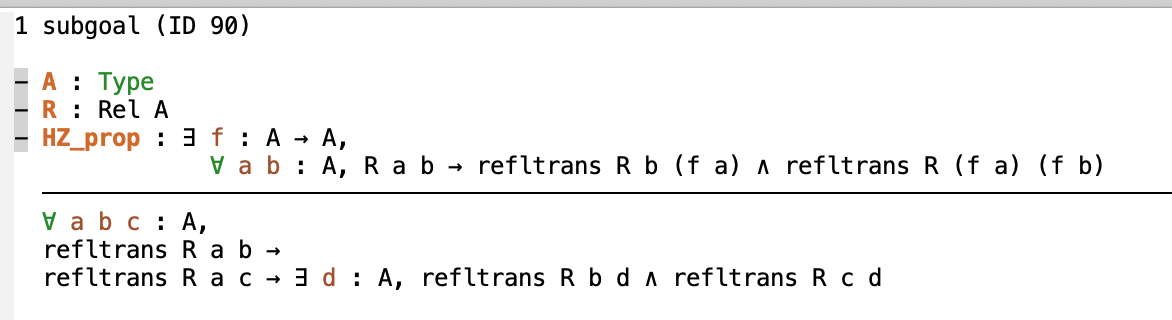
\includegraphics[scale=0.5]{figs/fig3.png} } \begin{coqdoccode}
\coqdocemptyline
\coqdocindent{1.00em}
\coqdoctac{intros} \coqdocvar{a} \coqdocvar{b} \coqdocvar{c} \coqdocvar{Hrefl1} \coqdocvar{Hrefl2}. \end{coqdoccode}
\comm{Let $a, b$ and $c$ be elements of
     the set $A$, $Hrefl1$ the hypothesis that $a \tto_R b$, and
     $Hrefl2$ the hypothesis that $a\tto_R c$. We need to prove that
     there exists $d$ such that $b\tto_R d$ and $c\tto_R d$.} \begin{coqdoccode}
\coqdocemptyline
\coqdocindent{1.00em}
\coqdoctac{destruct} \coqdocvar{HZ\_prop} \coqdockw{as} [\coqdocvar{g} \coqdocvar{HZ\_prop}]. \end{coqdoccode}
\comm{We know from the hypothesis
     $HZ\_prop$ that there exists a mapping $f$ that is Z. Let's call
     $g$ this mapping, and we get following proof context:

      \symbol{92}includegraphics\coqdocvar{scale}=0.6\{figs/fig4.png\}

      The proof proceeds by nested induction, firstly on the length of
      the reduction from $a$ to $b$, and then on the length of the
      reduction from $a$ to $c$.} \begin{coqdoccode}
\coqdocemptyline
\coqdocindent{1.00em}
\coqdoctac{generalize} \coqdoctac{dependent} \coqdocvar{c}. \end{coqdoccode}
\comm{Before the first induction,
      i.e. induction on $Hrefl1$, the element $c$ needs to be
      generalized so that it can be afterwards instantiated with any
      reduct of $a$.} \begin{coqdoccode}
\coqdocemptyline
\coqdocindent{1.00em}
\coqdoctac{induction} \coqdocvar{Hrefl1}. \end{coqdoccode}
\comm{The induction on $Hrefl1$ corresponds to
       induction on the reflexive transitive closure of the relation
       $R$, and since $refltrans$ has two rules, the goal splits in
       two subgoals, one for each possible way of constructing $a
       \tto_R b$.} \begin{coqdoccode}
\coqdocemptyline
\coqdocindent{1.00em}
- \coqdoctac{intros} \coqdocvar{c} \coqdocvar{Hrefl2}. \end{coqdoccode}
\comm{In the first case, we have that $b = a$ since
    we are in the reflexive case. This means that we have to prove
    that there exists $d$, such that $a \tto_R d$ and $c \tto_R d$.} \begin{coqdoccode}
\coqdocemptyline
\coqdocindent{2.00em}
\coqdoctac{\ensuremath{\exists}} \coqdocvar{c}; \coqdoctac{split}. \end{coqdoccode}
\comm{Taking $d$ as $c$, the proof is simplified to $a
    \tto_R c$ and $c \tto_R c$.} \begin{coqdoccode}
\coqdocemptyline
\coqdocindent{2.00em}
+ \coqdoctac{assumption}. \end{coqdoccode}
\comm{The first component is exactly the hypothesis
        $Hrefl2$ and } \begin{coqdoccode}
\coqdocemptyline
\coqdocindent{2.00em}
+ \coqdoctac{apply} \coqdocvar{refl}. \end{coqdoccode}
\comm{$c \tto_R c$ corresponds to an application of
        the $refl$ axiom.} 

 The interesting part of the proof is then given by the
        inductive case, i.e. when $a\tto_R b$ is generated by the rule
        (\coqdocvar{rtrans}). In this case, the reduction from \coqdocvar{a} to \coqdocvar{b} is
        done in at least one step, therefore there must exists an
        element $a'$ such that the following diagram holds.


         \[\xymatrix{ & & a \ar@{->}[dl] \ar@{->>}[dr] & \\ & a'
        \ar@{->>}[dl] & & c \ar@{.>>}[ddll] \\ b \ar@{.>>}[dr] & & &
        \\ & d & & }\]  


        

        The induction hypothesis states that every divergence from
        $a'$ that reduces to $b$ from one side converges: \coqdocvar{IHHrefl1}
        : $\forall c_0 : A, a'\tto_R c_0 \to (\exists d : A, b\tto_R d
        \land c_0\tto_R d$). Now, we'd like apply induction on the
        hypothesis \coqdocvar{Hrefl2} (a\symbol{92}tto\_R c), but the current proof context has the
        hypothesis \coqdocvar{H}: $a\to_R a'$ (\coqdocvar{a} reduces to \coqdocvar{a'} in one step),
        and hence it is the sole hypothesis depending on \coqdocvar{a} in the
        current proof context. If we were to apply induction on \coqdocvar{Hrefl2} now, 
        the generated induction hypothesis \coqdocvar{IHrefl2} would assume that there is 
        a term $a''$ such that $a \to_R a'' \tto_R c$ and would require that 
        $a'' \to_R a'$, which is generally false. In order to circumvent 
        this problem, we need to discard the hypothesis \coqdocvar{H} from our proof 
        context, and replace it by another relevant information derived from 
        the Z property as shown in what follows. \begin{coqdoccode}
\coqdocemptyline
\coqdocindent{1.00em}
- \coqdoctac{intros} \coqdocvar{c0} \coqdocvar{Hrefl2}. \end{coqdoccode}
\comm{Let $c_0$ be a reduct of $a$, and $Hrefl2$
    be the hypothesis $a \tto_R c_0$. So the reduction $a\tto_R c$ in
    the above diagram is now $a\tto_R c_0$ due to a renaming of
    variables automatically done by the Coq system. In addition, the
    reduction $a \to_R a' \tto_R b$ is now $a\to_R b \tto_R c$, as
    shown below:

    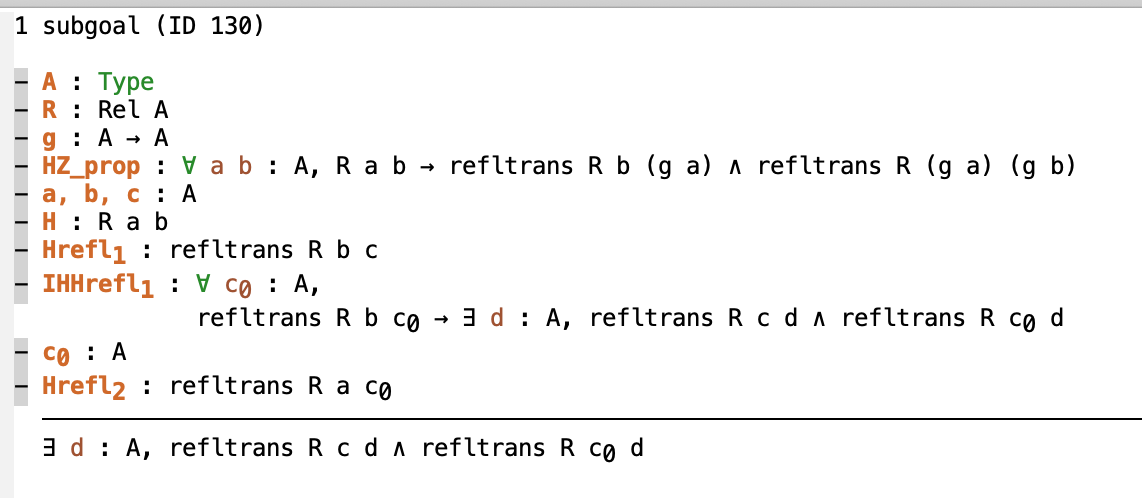
\includegraphics[scale=0.5]{figs/fig5-1.png}

    Before applying induction to $Hrefl2$: $a \tto_R c_0$, we will derive 
    $b\tto_R (g\ a)$ and $a\tto_R (g\ a)$ from the proof context so we can
    discard the hypothesis $H$: $a\to_R$.} \begin{coqdoccode}
\coqdocemptyline
\coqdocindent{2.00em}
\coqdoctac{assert} (\coqdocvar{Hbga}: \coqdocvar{refltrans} \coqdocvar{R} \coqdocvar{b} (\coqdocvar{g} \coqdocvar{a})).\coqdoceol
\coqdocindent{2.00em}
\{ \coqdoctac{apply} \coqdocvar{HZ\_prop}; \coqdoctac{assumption}. \} \end{coqdoccode}
\comm{We call $Hbga$ the reduction
    $b\tto_R (g\ a)$ that is directly obtained from the Z property.} \begin{coqdoccode}
\coqdocnoindent
\coqdoceol
\coqdocindent{2.00em}
\coqdoctac{assert} (\coqdocvar{Haga}: \coqdocvar{refltrans} \coqdocvar{R} \coqdocvar{a} (\coqdocvar{g} \coqdocvar{a})).\coqdoceol
\coqdocindent{2.00em}
\{ \coqdoctac{apply} \coqdocvar{rtrans} \coqdockw{with} \coqdocvar{b}; \coqdoctac{assumption}. \} \end{coqdoccode}
\comm{Call $Haga$ the
        reduction $a\tto_R (g\ a)$, and prove it using the
        transitivity of $\tto_R$, since $a \to_R b$ and $b \tto_R (g\
        a)$. Diagrammatically, we change from the situation on the
        top to the bottomone on the right:

        \xymatrix{ & & a \ar@{->>}[ddrr]_R \ar@{->}[dl]^R & & \\ & b
        \ar@{->>}[dl]^R & & & \\ c \ar@{.>>}[ddrr]_R & & & & c_0
        \ar@{.>>}[ddll]^R \\ & & & & \\ & & d & & } 

        \xymatrix{ & & a \ar@{->>}[ddrr]_R \ar@{->>}[dd]_R & & \\ & b
        \ar@{->>}[dl]^R \ar@{->>}[dr]_R & & & \\ c \ar@{.>>}[ddrr]_R &
        & (g \; a) & & c_0 \ar@{.>>}[ddll]^R \\ & & & & \\ & & d & &} } \begin{coqdoccode}
\coqdocnoindent
\coqdoceol
\coqdocindent{2.00em}
\coqdoctac{clear} \coqdocvar{H}. \coqdoctac{generalize} \coqdoctac{dependent} \coqdocvar{b}. \end{coqdoccode}
\comm{At this point we can remove
      the hypothesis $H$ from the context, and generalize $b$. Doing so, 
      we generalize $IHHrefl1$, which, in conjunction with the hypotheses 
      that depend on a (namely, $Hrefl2$, $Hbga$, and $Haga$), will form 
      the four necessary conditions for use of the second inductive 
      hypothesis, $IHHrefl2$.} \begin{coqdoccode}
\coqdocemptyline
\coqdocindent{2.00em}
\coqdoctac{induction} \coqdocvar{Hrefl2}. \end{coqdoccode}
\comm{Now we are ready to start the induction on
    the reduction $a\tto_R c_0$, and we have two subgoals.} \begin{coqdoccode}
\coqdocemptyline
\coqdocindent{2.00em}
+ \coqdoctac{intros} \coqdocvar{b} \coqdocvar{Hrefl1} \coqdocvar{IHHrefl1} \coqdocvar{Hbga}. \end{coqdoccode}
\comm{The first subgoal corresponds
        to the reflexive case that is closed by the induction
        hypothesis $IHHrefl1$:

        \[\xymatrix{ & & a \ar@{->>}[dd]^{H2} & & \\ & b
        \ar@{->>}[dl]_{Hrefl1} \ar@{->>}[dr]^{H1} & & & \\ c
        \ar@{.>>}[dr] & IHHrefl1 & (g \; a) \ar@{.>>}[dl] & & \\ & d &
        &&}\] } \begin{coqdoccode}
\coqdocemptyline
\coqdocindent{3.00em}
\coqdoctac{assert} (\coqdocvar{IHHrefl1\_ga} := \coqdocvar{IHHrefl1} (\coqdocvar{g} \coqdocvar{a}));\coqdoceol
\coqdocindent{4.00em}
\coqdoceol
\coqdocindent{4.00em}
\coqdoctac{apply} \coqdocvar{IHHrefl1\_ga} \coqdoctac{in} \coqdocvar{Hbga}. \end{coqdoccode}
\comm{In order to apply $IHHrefl1$, we instantiate $c_0$ with $(g\
      a)$.} \begin{coqdoccode}
\coqdocemptyline
\coqdocindent{3.00em}
\coqdoctac{destruct} \coqdocvar{Hbga}. \end{coqdoccode}
\comm{Therefore, there exists an element, say $x$,
      such that both $c\tto_R x$ and $(g\ a) \tto_R x$.} \begin{coqdoccode}
\coqdocemptyline
\coqdocindent{3.00em}
\coqdoctac{\ensuremath{\exists}} \coqdocvar{x}; \coqdoctac{split}. \end{coqdoccode}
\comm{We then take $x$ to show that $c\tto_R x$ and $a
      \tto_R x$.} \begin{coqdoccode}
\coqdocemptyline
\coqdocindent{3.00em}
\ensuremath{\times} \coqdoctac{apply} \coqdocvar{H}. \end{coqdoccode}
\comm{Note that $c\tto_R x$ is already an hypothesis,
        and we are done.} \begin{coqdoccode}
\coqdocemptyline
\coqdocindent{3.00em}
\ensuremath{\times} \coqdoctac{apply} \coqdocvar{refltrans\_composition} \coqdockw{with} (\coqdocvar{g} \coqdocvar{a});\coqdoceol
\coqdocnoindent
\coqdoceol
\coqdocindent{4.00em}
[\coqdoctac{assumption} \ensuremath{|} \coqdoctac{apply} \coqdocvar{H}]. \end{coqdoccode}
      \comm{The proof of $a \tto_R x$ is done by the transitivity of
      $\tto_R$ taking $(g\ a)$ as the intermediate step.} \begin{coqdoccode}
\coqdocemptyline
\coqdocindent{2.00em}
+ \coqdoctac{intros} \coqdocvar{b0} \coqdocvar{Hrefl1} \coqdocvar{IHHrefl1} \coqdocvar{Hb0ga}. \end{coqdoccode}
\comm{The second subgoal corresponds
        to the case in which $a\tto_R c_0$ is generated by the rule
        $(rtrans)$. Therefore, there exists a term $b$ such that
        $a\to_R b$ and $b \tto_R c_0$. The corresponding proof context
        after introducing the universally quantified variable $b0$,
        the hypothesis $Hrefl1$ and the induction hypothesis
        $IHHrefl1$ generated by the first outer induction and the fact
        that $b0 \tto_R (g\ a)$ is given by:

        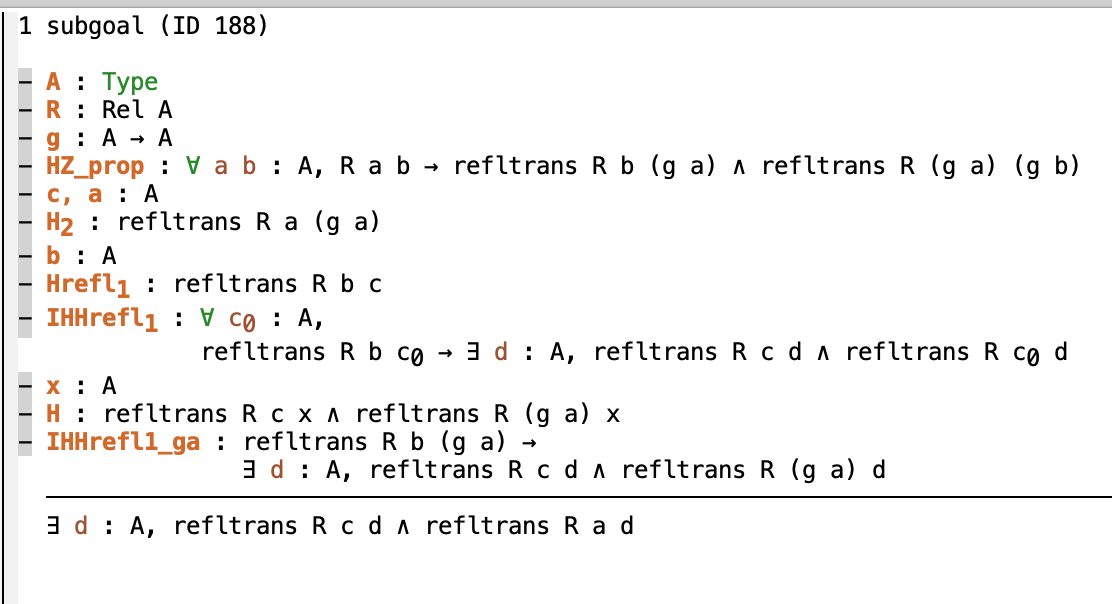
\includegraphics[scale=0.48]{figs/fig7.png} } \begin{coqdoccode}
\coqdocemptyline
\coqdocindent{3.00em}
\coqdoctac{apply} \coqdocvar{IHHrefl2} \coqdockw{with} \coqdocvar{b0}. \end{coqdoccode}
\comm{The second goal, i.e. the inductive case is 
      the consequent on $IHHrefl2$, so we can apply $IHHrefl2$ to prove it. Doing so, 
      we must prove the antecedent of $IHHrefl2$, which consists of four separate 
      hypotheses that we must prove. Those hypotheses are as follows:} \begin{coqdoccode}
\coqdocemptyline
\coqdocindent{3.00em}
\ensuremath{\times} \coqdoctac{apply} \coqdocvar{refltrans\_composition} \coqdockw{with} (\coqdocvar{g} \coqdocvar{a});\coqdoceol
\coqdocindent{5.00em}
\coqdoceol
\coqdocindent{4.00em}
\coqdoctac{apply} \coqdocvar{HZ\_prop}; \coqdoctac{assumption}. \end{coqdoccode}
\comm{1. $b \tto_R (g\ b)$: This is proved by the transitivity of the
      reflexive transitive closure of $R$ using the
      hypothesis (H: $a\to_R b$) and $HZ\_prop$: $\forall a\
      b: a \to_R b \to (b \tto_R (g\ a) \land (g\ a) \tto_R (g\ b))$.} \begin{coqdoccode}
\coqdocemptyline
\coqdocindent{3.00em}
\ensuremath{\times} \coqdoctac{assumption}. \end{coqdoccode}
\comm{2. $b0 \tto_R c$: This is exactly the
          hypothesis $Hrefl1$.} \begin{coqdoccode}
\coqdocemptyline
\coqdocindent{3.00em}
\ensuremath{\times} \coqdoctac{assumption}. \end{coqdoccode}
\comm{3. $\forall c0: b0 \tto_R c0 \to (\exists d:
            c \tto_R d \land c0 \tto_R d)$: This is exactly the
            induction hypothesis $IHHrefl1$.} \begin{coqdoccode}
\coqdocemptyline
\coqdocindent{3.00em}
\ensuremath{\times} \coqdoctac{apply} \coqdocvar{refltrans\_composition} \coqdockw{with} (\coqdocvar{g} \coqdocvar{a});\coqdoceol
\coqdocindent{4.00em}
[ \coqdoctac{assumption} \ensuremath{|} \coqdoctac{apply} \coqdocvar{HZ\_prop}; \coqdoctac{assumption}]. \end{coqdoccode}
\comm{4. $b0 \tto_R (g\ b)$: This is proved by the transitivity of
      the reflexive transitive closure of $R$ using the
      hypothesis $H'$: $b0 \tto_R (g\ a)$ and the fact that
      $(g\ a) \tto_R (g\ b)$ that is obtained from the fact that
      $R$ satisfies the Z property (hypothesis
      $HZ\_prop$).} \begin{coqdoccode}
\coqdocemptyline
\coqdocnoindent
\coqdockw{Qed}.\coqdoceol
\coqdocemptyline
\coqdocemptyline
\end{coqdoccode}
An alternative proof that Z implies confluence is possible via the
    notion of semiconfluence, which is equivalent to confluence, as
    done in \cite{zproperty}. Unlike the proof in \cite{zproperty} and 
    similarly to our previous proof, our proof of the Theorem that 
    Z implies semiconfluence is constructive, but we
    will not explain it here due to lack of space; any
    interested reader can find it in the Coq file in our GitHub
    repository. \begin{coqdoccode}
\coqdocemptyline
\coqdocnoindent
\coqdockw{Definition} \coqdocvar{SemiConfl} \{\coqdocvar{A}:\coqdockw{Type}\} (\coqdocvar{R}: \coqdocvar{Rel} \coqdocvar{A}) := \coqdockw{\ensuremath{\forall}} \coqdocvar{a} \coqdocvar{b} \coqdocvar{c}, \coqdocvar{R} \coqdocvar{a} \coqdocvar{b} \ensuremath{\rightarrow} (\coqdocvar{refltrans} \coqdocvar{R}) \coqdocvar{a} \coqdocvar{c} \ensuremath{\rightarrow} (\coqdoctac{\ensuremath{\exists}} \coqdocvar{d}, (\coqdocvar{refltrans} \coqdocvar{R}) \coqdocvar{b} \coqdocvar{d} \ensuremath{\land} (\coqdocvar{refltrans} \coqdocvar{R}) \coqdocvar{c} \coqdocvar{d}).\coqdoceol
\coqdocemptyline
\coqdocnoindent
\coqdockw{Theorem} \coqdocvar{Z\_prop\_implies\_SemiConfl} \{\coqdocvar{A}:\coqdockw{Type}\}: \coqdockw{\ensuremath{\forall}} \coqdocvar{R}: \coqdocvar{Rel} \coqdocvar{A}, \coqdocvar{Z\_prop} \coqdocvar{R} \ensuremath{\rightarrow} \coqdocvar{SemiConfl} \coqdocvar{R}.\coqdoceol
\coqdocemptyline
\coqdocnoindent
\coqdockw{Theorem} \coqdocvar{Semi\_equiv\_Confl} \{\coqdocvar{A}: \coqdockw{Type}\}: \coqdockw{\ensuremath{\forall}} \coqdocvar{R}: \coqdocvar{Rel} \coqdocvar{A}, \coqdocvar{Confl} \coqdocvar{R} \ensuremath{\leftrightarrow} \coqdocvar{SemiConfl} \coqdocvar{R}.\coqdoceol
\coqdocemptyline
\coqdocnoindent
\coqdockw{Corollary} \coqdocvar{Zprop\_implies\_Confl\_via\_SemiConfl} \{\coqdocvar{A}:\coqdockw{Type}\}: \coqdockw{\ensuremath{\forall}} \coqdocvar{R}: \coqdocvar{Rel} \coqdocvar{A}, \coqdocvar{Z\_prop} \coqdocvar{R} \ensuremath{\rightarrow} \coqdocvar{Confl} \coqdocvar{R}.\coqdoceol
\coqdocnoindent
\coqdockw{Proof}. \coqdoctac{intros} \coqdocvar{R} \coqdocvar{HZ\_prop}. \coqdoctac{apply} \coqdocvar{Semi\_equiv\_Confl}. \coqdoctac{generalize} \coqdoctac{dependent} \coqdocvar{HZ\_prop}.\coqdoceol
\coqdocindent{3.50em}
\coqdoctac{apply} \coqdocvar{Z\_prop\_implies\_SemiConfl}. \coqdockw{Qed}.\coqdoceol
\coqdocemptyline
\end{coqdoccode}
\section{An extension of the Z property: Compositional Z}




    In this section we present a formalization of an extension of the
    Z property with compositional functions, known as \textit{Compositional
    Z}, as presented in \cite{Nakazawa-Fujita2016}. The
    compositional Z is an interesting property because it allows a
    kind of modular approach to the Z property in such a way that the
    reduction relation can be split into two parts. More precisely,
    given an ARS $(A,\to_R)$, one must be able to decompose the
    relation $\to_R$ into two parts, say $\to_1$ and $\to_2$ such that
    $\to_R = \to_1\cup \to_2$. This kind of decomposition can be done
    in several interesting situations such as the $\lambda$-calculus
    with $\beta\eta$-reduction\cite{Ba84}, extensions of the
    $\lambda$-calculus with explicit substitutions\cite{accl91}, the
    $\lambda\mu$-calculus\cite{Parigot92}, etc. But before
    presenting the full definition of the Compositional Z, we need
    to define the \textit{weak Z property}:


    \begin{figure}[h] \centering \[ \xymatrix{ a \ar[r]_R & b
        \ar@{.>>}[dl]^x\\ f(a) \ar@{.>>}[r]_x & f(b) \\ } \]
        \caption{The weak Z property}\label{fig:weakZ} \end{figure}


    \begin{definition} Let $(A,\to_R)$ be an ARS and $\to_R'$ a
     relation on $A$. A mapping $f$ satisfies the {\it weak Z
     property} for $\to_R$ by $\to_R'$ if $a\to_R b$ implies $b \tto_R'
     f(a)$ and $f(a) \tto_R' f(b)$ (cf. Figure
     \ref{fig:weakZ}). Therefore, a mapping $f$ satisfies the Z
     property for $\to_R$ if it satisfies the weak Z property by
     itself.  \end{definition}


    When $f$ satisfies the weak Z property, we also say that $f$ is
    weakly Z, and the corresponding definition in Coq is given as
    follows: \begin{coqdoccode}
\coqdocemptyline
\coqdocnoindent
\coqdockw{Definition} \coqdocvar{f\_is\_weak\_Z} \{\coqdocvar{A}\} (\coqdocvar{R} \coqdocvar{R'}: \coqdocvar{Rel} \coqdocvar{A}) (\coqdocvar{f}: \coqdocvar{A} \ensuremath{\rightarrow} \coqdocvar{A}) := \coqdockw{\ensuremath{\forall}} \coqdocvar{a} \coqdocvar{b}, \coqdocvar{R} \coqdocvar{a} \coqdocvar{b} \ensuremath{\rightarrow} ((\coqdocvar{refltrans} \coqdocvar{R'}) \coqdocvar{b} (\coqdocvar{f} \coqdocvar{a}) \ensuremath{\land} (\coqdocvar{refltrans} \coqdocvar{R'}) (\coqdocvar{f} \coqdocvar{a}) (\coqdocvar{f} \coqdocvar{b})).\coqdoceol
\coqdocemptyline
\end{coqdoccode}
The compositional Z is an extension of the Z property for
compositional functions, where composition is defined as usual: \begin{coqdoccode}
\coqdocemptyline
\coqdocnoindent
\coqdockw{Definition} \coqdocvar{comp} \{\coqdocvar{A}\} (\coqdocvar{f1} \coqdocvar{f2}: \coqdocvar{A} \ensuremath{\rightarrow} \coqdocvar{A}) := \coqdockw{fun} \coqdocvar{x}:\coqdocvar{A} \ensuremath{\Rightarrow} \coqdocvar{f1} (\coqdocvar{f2} \coqdocvar{x}).\coqdoceol
\coqdocnoindent
\coqdockw{Notation} "f1 \# f2" := (\coqdocvar{comp} \coqdocvar{f1} \coqdocvar{f2}) (\coqdoctac{at} \coqdockw{level} 40).\coqdoceol
\coqdocemptyline
\end{coqdoccode}
\noindent and the disjoint union is inductively defined as: \begin{coqdoccode}
\coqdocemptyline
\coqdocnoindent
\coqdockw{Inductive} \coqdocvar{union} \{\coqdocvar{A}\} (\coqdocvar{red1} \coqdocvar{red2}: \coqdocvar{Rel} \coqdocvar{A}) : \coqdocvar{Rel} \coqdocvar{A} :=\coqdoceol
\coqdocnoindent
\ensuremath{|} \coqdocvar{union\_left}: \coqdockw{\ensuremath{\forall}} \coqdocvar{a} \coqdocvar{b}, \coqdocvar{red1} \coqdocvar{a} \coqdocvar{b} \ensuremath{\rightarrow} \coqdocvar{union} \coqdocvar{red1} \coqdocvar{red2} \coqdocvar{a} \coqdocvar{b}\coqdoceol
\coqdocnoindent
\ensuremath{|} \coqdocvar{union\_right}: \coqdockw{\ensuremath{\forall}} \coqdocvar{a} \coqdocvar{b}, \coqdocvar{red2} \coqdocvar{a} \coqdocvar{b} \ensuremath{\rightarrow} \coqdocvar{union} \coqdocvar{red1} \coqdocvar{red2} \coqdocvar{a} \coqdocvar{b}.\coqdoceol
\coqdocnoindent
\coqdockw{Notation} "R1 !\_! R2" := (\coqdocvar{union} \coqdocvar{R1} \coqdocvar{R2}) (\coqdoctac{at} \coqdockw{level} 40).\coqdoceol
\coqdocemptyline
\coqdocemptyline
\end{coqdoccode}
We are now ready to present the definition of the compositional Z:


    \begin{theorem}\cite{Nakazawa-Fujita2016}\label{thm:zcomp} Let
     $(A,\to_R)$ be an ARS such that $\to_R = \to_1 \cup \to_2$. If
     there exists mappings $f_1,f_2: A \to A$ such that
     \begin{enumerate} \item $f_1$ is Z for $\to_1$ \item $a \to_1 b$
     implies $f_2(a) \tto f_2(b)$ \item $a \tto f_2(a)$ holds for any
     $a\in Im(f_1)$ \item $f_2 \circ f_1$ is weakly Z for $\to_2$ by
     $\to_R$ \end{enumerate} then $f_2 \circ f_1$ is Z for
     $(A,\to_R)$, and hence $(A,\to_R)$ is confluent.  \end{theorem}


    We define the predicate \coqdocvar{Z\_comp} that corresponds to the premises
    of Theorem \ref{thm:zcomp}, i.e. to the conjunction of items
    (i), (ii), (iii) and (iv) in addition to the fact that $\to_R =
    \to_1 \cup \to_2$, where $\to_1$ (resp. $\to_2$) is written as
    \coqdocvar{R1} (resp. \coqdocvar{R2}): \begin{coqdoccode}
\coqdocemptyline
\coqdocnoindent
\coqdockw{Definition} \coqdocvar{Z\_comp} \{\coqdocvar{A}:\coqdockw{Type}\} (\coqdocvar{R} :\coqdocvar{Rel} \coqdocvar{A}) := \coqdoctac{\ensuremath{\exists}} (\coqdocvar{R1} \coqdocvar{R2}: \coqdocvar{Rel} \coqdocvar{A}) (\coqdocvar{f1} \coqdocvar{f2}: \coqdocvar{A} \ensuremath{\rightarrow} \coqdocvar{A}), \coqdocvar{R} = (\coqdocvar{R1} !\coqdocvar{\_}! \coqdocvar{R2}) \ensuremath{\land} \coqdocvar{f\_is\_Z} \coqdocvar{R1} \coqdocvar{f1} \ensuremath{\land} (\coqdockw{\ensuremath{\forall}} \coqdocvar{a} \coqdocvar{b}, \coqdocvar{R1} \coqdocvar{a} \coqdocvar{b} \ensuremath{\rightarrow} (\coqdocvar{refltrans} \coqdocvar{R}) (\coqdocvar{f2} \coqdocvar{a}) (\coqdocvar{f2} \coqdocvar{b})) \ensuremath{\land} (\coqdockw{\ensuremath{\forall}} \coqdocvar{a} \coqdocvar{b}, \coqdocvar{b} = \coqdocvar{f1} \coqdocvar{a} \ensuremath{\rightarrow} (\coqdocvar{refltrans} \coqdocvar{R}) \coqdocvar{b} (\coqdocvar{f2} \coqdocvar{b})) \ensuremath{\land} (\coqdocvar{f\_is\_weak\_Z} \coqdocvar{R2} \coqdocvar{R} (\coqdocvar{f2} \# \coqdocvar{f1})).\coqdoceol
\coqdocemptyline
\coqdocemptyline
\end{coqdoccode}
As stated by Theorem \ref{thm:zcomp}, the compositional Z gives
    a sufficient condition for compositional functions to be Z. In
    other words, compositional Z implies Z, which is justified by the
    diagrams of Figure \ref{fig:zcomp}.


    \begin{figure}[h]\begin{tabular}{l@{\hskip 3cm}l} $\xymatrix{ a
    \ar@{->}[rr]^1 && b \ar@{.>>}[dll]_1\\ f_1(a)\ar@{.>>}[d]
    \ar@{.>>}[rr]^1 && f_1(b) \\ f_2(f_1(a)) \ar@{.>>}[rr] &&
    f_2(f_1(b)) }$ & $\xymatrix{ a \ar@{->}[rr]^2 && b
    \ar@{.>>}[ddll]\\ & & \\ f_2(f_1(a)) \ar@{.>>}[rr] && f_2(f_1(b))
    }$ \end{tabular}\caption{Compositional Z implies
    Z}\label{fig:zcomp}\end{figure}


    In what follows, we present our commented Coq proof of this fact:
    \begin{coqdoccode}
\coqdocemptyline
\coqdocnoindent
\coqdockw{Theorem} \coqdocvar{Z\_comp\_implies\_Z\_prop} \{\coqdocvar{A}:\coqdockw{Type}\}: \coqdockw{\ensuremath{\forall}} (\coqdocvar{R} :\coqdocvar{Rel} \coqdocvar{A}), \coqdocvar{Z\_comp} \coqdocvar{R} \ensuremath{\rightarrow} \coqdocvar{Z\_prop} \coqdocvar{R}.\coqdoceol
\coqdocnoindent
\coqdockw{Proof}.\coqdoceol
\coqdocindent{1.00em}
\coqdoctac{intros} \coqdocvar{R} \coqdocvar{H}. \end{coqdoccode}
\comm{Let $R$ be a relation over $A$, and $H$ the
      hypothesis that $R$ satisfies the compositional Z.} \begin{coqdoccode}
\coqdocemptyline
\coqdocindent{1.00em}
\coqdoctac{unfold} \coqdocvar{Z\_prop}. \coqdoctac{unfold} \coqdocvar{Z\_comp} \coqdoctac{in} \coqdocvar{H}. \coqdoctac{destruct} \coqdocvar{H} \coqdockw{as}\coqdoceol
\coqdocindent{1.00em}
[ \coqdocvar{R1} [ \coqdocvar{R2} [\coqdocvar{f1} [\coqdocvar{f2} [\coqdocvar{Hunion} [\coqdocvar{H1} [\coqdocvar{H2} [\coqdocvar{H3} \coqdocvar{H4}]]]]]]]]. \end{coqdoccode}
\comm{Now
      unfold the definitions of $Z\_prop$ and $Z\_comp$ as presented
      before, and name the hypothesis of the compositional Z as in
      Theorem \ref{thm:zcomp}. We need to prove that there exists a
      map, say $f$, that is Z as shown by the current proof context:
      \newline

      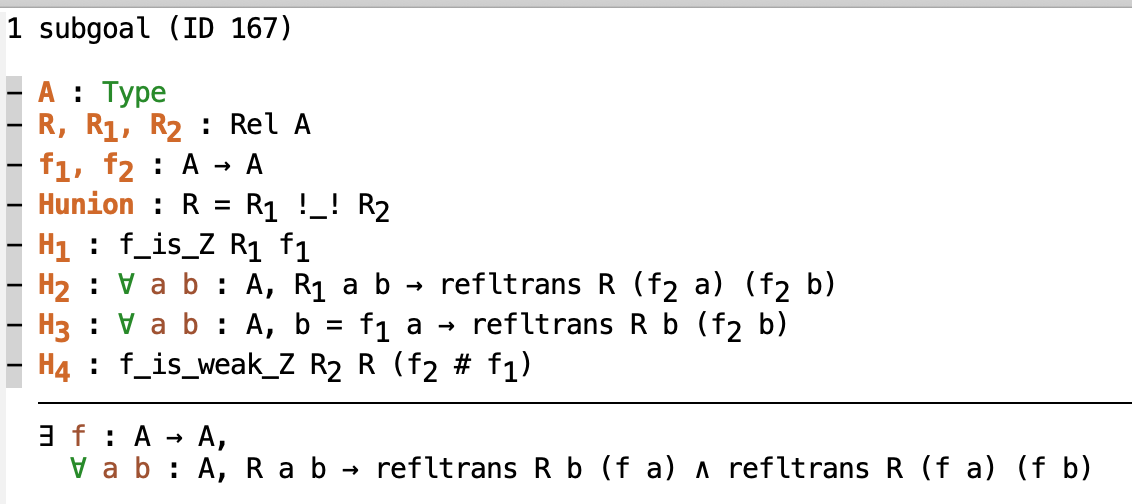
\includegraphics[scale=0.4]{figs/fig8.png} } \begin{coqdoccode}
\coqdocemptyline
\coqdocindent{1.00em}
\coqdoctac{\ensuremath{\exists}} (\coqdocvar{f2} \# \coqdocvar{f1}). \end{coqdoccode}
\comm{We will prove that the composition $f_2 \circ f_1$
  is Z.} \begin{coqdoccode}
\coqdocemptyline
\coqdocindent{1.00em}
\coqdoctac{intros} \coqdocvar{a} \coqdocvar{b} \coqdocvar{HR}. \end{coqdoccode}
\comm{Let $a$ and $b$ be elements of $A$, and suppose
  that $a$ $R$-reduces to $b$ in one step, i.e. that $a \to_R b$ and
  call $HR$ this hypothesis.} \begin{coqdoccode}
\coqdocemptyline
\coqdocindent{1.00em}
\coqdoctac{inversion} \coqdocvar{Hunion}; \coqdoctac{subst}. \coqdoctac{clear} \coqdocvar{H}. \coqdoctac{inversion} \coqdocvar{HR}; \coqdoctac{subst}. \end{coqdoccode}
\comm{Since
  $R$ is the union of $R1$ and $R2$, one has that $a$ reduces to $b$
  in one step via either $R1$ or $R2$. Therefore, there are two cases
  to consider:} \begin{coqdoccode}
\coqdocemptyline
\coqdocindent{1.00em}
- \coqdoctac{split}. \end{coqdoccode}
\comm{Firstly, suppose that $a$ $R1$-reduces in one step to
    $b$, i.e. $a \to_{R1} b$.} \begin{coqdoccode}
\coqdocemptyline
\coqdocindent{2.00em}
+ \coqdoctac{apply} \coqdocvar{refltrans\_composition} \coqdockw{with} (\coqdocvar{f1} \coqdocvar{a}). \end{coqdoccode}
\comm{In order to prove
    that $b \tto_R (f_2 (f_1\ a))$, we first need to show that $b
    \tto_{R1} (f_1\ a)$, and then that $(f_1\ a) \tto_R (f_2 (f_1\ a))$ as
    shown in Figure \ref{fig:zcomp}.} \begin{coqdoccode}
\coqdocemptyline
\coqdocindent{3.00em}
\ensuremath{\times} \coqdoctac{apply} \coqdocvar{H1} \coqdoctac{in} \coqdocvar{H}. \coqdoctac{destruct} \coqdocvar{H}. \coqdoctac{apply} \coqdocvar{refltrans\_union}; \coqdoctac{assumption}. \end{coqdoccode}
    \comm{The proof of $b \tto_{R1} (f_1\ a)$ is done from the fact that $f_1$
    is Z for $R1$.} \begin{coqdoccode}
\coqdocemptyline
\coqdocindent{3.00em}
\ensuremath{\times} \coqdoctac{apply} \coqdocvar{H3} \coqdockw{with} \coqdocvar{a}; \coqdoctac{reflexivity}. \end{coqdoccode}
\comm{The proof that $(f_1\ a)
    \tto_R (f_2 (f_1\ a))$ is a direct consequence of the hypothesis
    $H3$.} \begin{coqdoccode}
\coqdocemptyline
\coqdocindent{2.00em}
+ \coqdoctac{apply} \coqdocvar{H1} \coqdoctac{in} \coqdocvar{H}. \coqdoctac{destruct} \coqdocvar{H}. \coqdoctac{clear} \coqdocvar{H} \coqdocvar{HR}. \coqdoctac{unfold} \coqdocvar{comp}. \end{coqdoccode}
\comm{The
    proof that $(f_2 (f_1\ a))$ $R$-reduces to $(f_2 (f_1\ b))$ is
    more tricky. Initially, note that, since $a \to_{R1} b$ then we
    get that $(f_1\ a) \tto_{R1} (f_1\ b)$ by the Z property.} \begin{coqdoccode}
\coqdocemptyline
\coqdocindent{3.00em}
\coqdoctac{induction} \coqdocvar{H0}. \end{coqdoccode}
\comm{Now, the goal can be obtained from $H2$ as
      long as $(f_1\ a) \to_{R1} (f_1\ b)$, but from the hypothesis
      $H0$ we have that $(f_1\ a) \tto_{R1} (f_1\ b)$. Therefore, we
      proceed by induction on $H0$.} \begin{coqdoccode}
\coqdocemptyline
\coqdocindent{3.00em}
\ensuremath{\times} \coqdoctac{apply} \coqdocvar{refl}. \end{coqdoccode}
\comm{The reflexive case is trivial because $a$ and
        $b$ are equal.} \begin{coqdoccode}
\coqdocemptyline
\coqdocindent{3.00em}
\ensuremath{\times} \coqdoctac{apply} \coqdocvar{refltrans\_composition}\coqdoceol
\coqdocindent{7.00em}
\coqdoceol
\coqdocindent{4.00em}
\coqdockw{with} (\coqdocvar{f2} \coqdocvar{b0}). \end{coqdoccode}
\comm{In the transitive case, we have that $(f_1\ a)$ $R1$-reduces to
        $(f_1\ b)$ in at least one step. The current proof context is
        as follows, up to renaming of variables:

        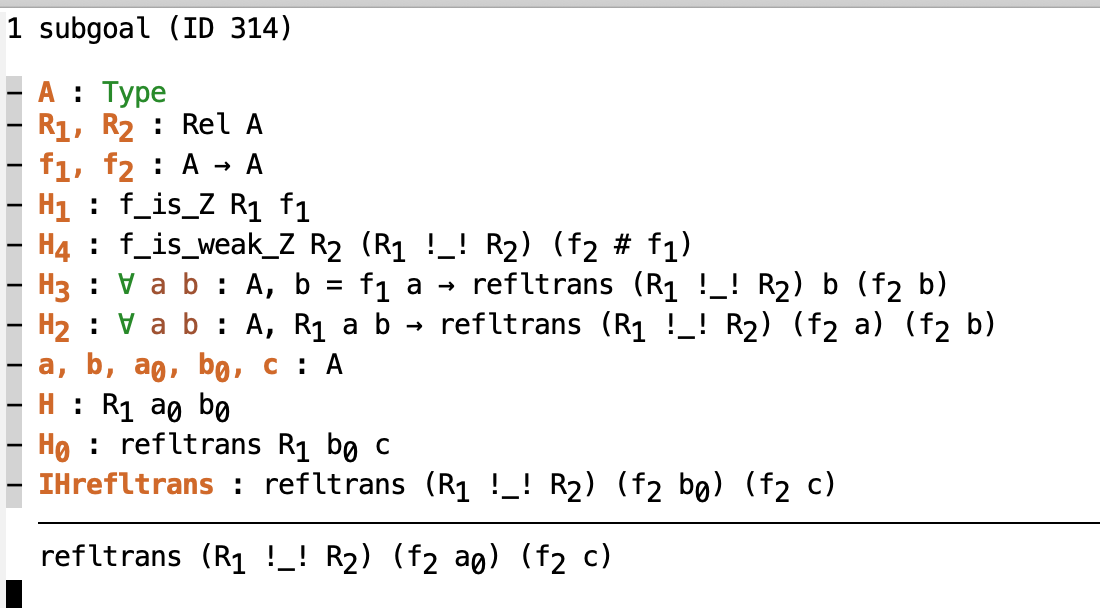
\includegraphics[scale=0.5]{figs/fig9.png}

      Therefore, there exists some element $b0$ such that $a0\to_{R1}
      b0$ and $b0 \tto_{R1} c$ and we need to prove that $(f_2\ a0)
      \tto_{R1\cup R2} (f_2\ c)$. This can be done in two steps using
      the transitivity of [refltrans] taking $(f_2\ b0)$ as the
      intermediary term.} \begin{coqdoccode}
\coqdocemptyline
\coqdocindent{4.00em}
** \coqdoctac{apply} \coqdocvar{H2}; \coqdoctac{assumption}. \end{coqdoccode}
\comm{The first subgoal is then $(f_2\
           a0)\tto_{(R1 \cup R2)} (f_2\ b0)$ that is proved by
           hypothesis $H2$.} \begin{coqdoccode}
\coqdocemptyline
\coqdocindent{4.00em}
** \coqdoctac{assumption}. \end{coqdoccode}
\comm{And the second subgoal $(f_2\ b0) \tto_{(R1
           \cup R2)} (f_2\ c)$ is proved by the induction
           hypothesis.} \begin{coqdoccode}
\coqdocemptyline
\coqdocindent{1.00em}
- \coqdoctac{apply} \coqdocvar{H4}; \coqdoctac{assumption}. \end{coqdoccode}
\comm{Finally, when $a$ $R2$-reduces in one
    step to $b$ one concludes the proof using the assumption that
    $(f_2 \circ f_1)$ is weak Z.} \begin{coqdoccode}
\coqdocemptyline
\coqdocnoindent
\coqdockw{Qed}.\coqdoceol
\coqdocemptyline
\end{coqdoccode}
Now we can use the proofs of the theorems \coqdocvar{Z\_comp\_implies\_Z\_prop}
and \coqdocvar{Z\_prop\_implies\_Confl} to conclude that compositional Z is a
sufficient condition for confluence. \begin{coqdoccode}
\coqdocemptyline
\coqdocnoindent
\coqdockw{Corollary} \coqdocvar{Z\_comp\_is\_Confl} \{\coqdocvar{A}\}: \coqdockw{\ensuremath{\forall}} (\coqdocvar{R}: \coqdocvar{Rel} \coqdocvar{A}), \coqdocvar{Z\_comp} \coqdocvar{R} \ensuremath{\rightarrow} \coqdocvar{Confl} \coqdocvar{R}.\coqdoceol
\coqdocnoindent
\coqdockw{Proof}.\coqdoceol
\coqdocindent{1.00em}
\coqdoctac{intros} \coqdocvar{R} \coqdocvar{H}.\coqdoceol
\coqdocindent{1.00em}
\coqdoctac{apply} \coqdocvar{Z\_comp\_implies\_Z\_prop} \coqdoctac{in} \coqdocvar{H}.\coqdoceol
\coqdocindent{1.00em}
\coqdoctac{apply} \coqdocvar{Z\_prop\_implies\_Confl}; \coqdoctac{assumption}.\coqdoceol
\coqdocnoindent
\coqdockw{Qed}.\coqdoceol
\coqdocemptyline
\end{coqdoccode}
Rewriting Systems with equations is another interesting and
    non-trivial topic \cite{winkler89,terese03}. The confluence of
    rewriting systems with an equivalence relation can also be proved
    by a variant of the compositional Z, known as Z property
    modulo~\cite{AK12b}.


    \begin{theorem}\label{cor:zcomp} Let
     $(A,\to_R)$ be an ARS such that $\to_R = \to_1 \cup \to_2$. If
     there exist mappings $f_1,f_2: A \to A$ such that
     \begin{enumerate} \item $a \to_1 b$ implies $f_1(a) = f_1(b)$
     \item $a \tto_1 f_1(a), for all a$ \item $a \tto_R f_2(a)$ holds
     for any $a\in Im(f_1)$ \item $f_2 \circ f_1$ is weakly Z for
     $\to_2$ by $\to_R$ \end{enumerate} then $f_2 \circ f_1$ is Z for
     $(A,\to_R)$, and hence $(A,\to_R)$ is confluent. \end{theorem}


    We define the predicate \coqdocvar{Z\_comp\_eq} corresponding to the
    hypothesis of Theorem \ref{cor:zcomp}, and then we prove
    directly that if \coqdocvar{Z\_comp\_eq} holds for a relation \coqdocvar{R} then \coqdocvar{Zprop}
    \coqdocvar{R} also holds. This approach differs from
    \cite{Nakazawa-Fujita2016} that proves Theorem
    \ref{cor:zcomp}, which is a Corollary in \cite{Nakazawa-Fujita2016}, 
    directly from Theorem \ref{thm:zcomp} \begin{coqdoccode}
\coqdocemptyline
\coqdocnoindent
\coqdockw{Definition} \coqdocvar{Z\_comp\_eq} \{\coqdocvar{A}:\coqdockw{Type}\} (\coqdocvar{R} :\coqdocvar{Rel} \coqdocvar{A}) := \coqdoctac{\ensuremath{\exists}} (\coqdocvar{R1} \coqdocvar{R2}: \coqdocvar{Rel} \coqdocvar{A}) (\coqdocvar{f1} \coqdocvar{f2}: \coqdocvar{A} \ensuremath{\rightarrow} \coqdocvar{A}), \coqdocvar{R} = (\coqdocvar{R1} !\coqdocvar{\_}! \coqdocvar{R2}) \ensuremath{\land} (\coqdockw{\ensuremath{\forall}} \coqdocvar{a} \coqdocvar{b}, \coqdocvar{R1} \coqdocvar{a} \coqdocvar{b} \ensuremath{\rightarrow} (\coqdocvar{f1} \coqdocvar{a}) = (\coqdocvar{f1} \coqdocvar{b})) \ensuremath{\land} (\coqdockw{\ensuremath{\forall}} \coqdocvar{a}, (\coqdocvar{refltrans} \coqdocvar{R1}) \coqdocvar{a} (\coqdocvar{f1} \coqdocvar{a})) \ensuremath{\land} (\coqdockw{\ensuremath{\forall}} \coqdocvar{b} \coqdocvar{a}, \coqdocvar{a} = \coqdocvar{f1} \coqdocvar{b} \ensuremath{\rightarrow} (\coqdocvar{refltrans} \coqdocvar{R}) \coqdocvar{a} (\coqdocvar{f2} \coqdocvar{a})) \ensuremath{\land} (\coqdocvar{f\_is\_weak\_Z} \coqdocvar{R2} \coqdocvar{R} (\coqdocvar{f2} \# \coqdocvar{f1})).\coqdoceol
\coqdocemptyline
\coqdocnoindent
\coqdockw{Lemma} \coqdocvar{Z\_comp\_eq\_implies\_Z\_prop} \{\coqdocvar{A}:\coqdockw{Type}\}: \coqdockw{\ensuremath{\forall}} (\coqdocvar{R} : \coqdocvar{Rel} \coqdocvar{A}), \coqdocvar{Z\_comp\_eq} \coqdocvar{R} \ensuremath{\rightarrow} \coqdocvar{Z\_prop} \coqdocvar{R}.\coqdoceol
\coqdocnoindent
\coqdockw{Proof}.\coqdoceol
\coqdocindent{1.00em}
\coqdoctac{intros} \coqdocvar{R} \coqdocvar{Heq}. \coqdoctac{unfold} \coqdocvar{Z\_comp\_eq} \coqdoctac{in} \coqdocvar{Heq}. \end{coqdoccode}
\comm{Let $R$ be a relation
  and suppose that $R$ satisfies the predicate $Z\_comp\_eq$.} \begin{coqdoccode}
\coqdocemptyline
\coqdocindent{1.00em}
\coqdoctac{destruct} \coqdocvar{Heq} \coqdockw{as} [\coqdocvar{R1} [\coqdocvar{R2} [\coqdocvar{f1} [\coqdocvar{f2} [\coqdocvar{Hunion} [\coqdocvar{H1} [\coqdocvar{H2} [\coqdocvar{H3} \coqdocvar{H4}]]]]]]]]. \end{coqdoccode}
  \comm{Call $Hi$ the $i$th hypothesis as in \ref{cor:zcomp}.} \begin{coqdoccode}
\coqdocemptyline
\coqdocindent{1.00em}
\coqdoctac{unfold} \coqdocvar{Z\_prop}. \coqdoctac{\ensuremath{\exists}} (\coqdocvar{f2} \# \coqdocvar{f1}). \end{coqdoccode}
\comm{From the definition of the
  predicate $Z\_prop$, we need to find a map, say $f$ that is Z. Let
  $(f_2 \circ f_1)$ be such map.}  \begin{coqdoccode}
\coqdocemptyline
\coqdocindent{1.00em}
\coqdoctac{intros} \coqdocvar{a} \coqdocvar{b} \coqdocvar{Hab}. \end{coqdoccode}
\comm{In order to prove that $(f_2 \circ f_1)$ is Z,
  let $a$ and $b$ be arbitrary elements of type $A$, and $Hab$ be the
  hypothesis that $a \to_{R} b$.} \begin{coqdoccode}
\coqdocemptyline
\coqdocindent{1.00em}
\coqdoctac{inversion} \coqdocvar{Hunion}; \coqdoctac{subst}; \coqdoctac{clear} \coqdocvar{H}. \coqdoctac{inversion} \coqdocvar{Hab}; \coqdoctac{subst}; \coqdoctac{clear} \coqdocvar{Hab}. \end{coqdoccode}
  \comm{Since $a$ $R$-reduces in one step to $b$ and $R$ is the union of the
  relations $R1$ and $R2$ then we consider two cases:} \begin{coqdoccode}
\coqdocemptyline
\coqdocindent{1.00em}
- \coqdoctac{unfold} \coqdocvar{comp}; \coqdoctac{split}. \end{coqdoccode}
\comm{The first case is when $a \to_{R1}
    b$. This is equivalent to say that $f_2 \circ f_1$ is weak Z for
    $R1$ by $R1 \cup R2$.} \begin{coqdoccode}
\coqdocemptyline
\coqdocindent{2.00em}
+ \coqdoctac{apply} \coqdocvar{refltrans\_composition} \coqdockw{with} (\coqdocvar{f1} \coqdocvar{b}). \end{coqdoccode}
\comm{Therefore, we first
    prove that $b \tto_{(R1\cup R2)} (f_2 (f_1\ a))$, which can be
    reduced to $b \tto_{(R1\cup R2)} (f_1\ b)$ and $(f_1\ b)
    \tto_{(R1\cup R2)} (f_2 (f_1\ a))$ by the transitivity of
    $refltrans$.} \begin{coqdoccode}
\coqdocemptyline
\coqdocindent{3.00em}
\ensuremath{\times} \coqdoctac{apply} \coqdocvar{refltrans\_union}. \coqdoctac{apply} \coqdocvar{H2}. \end{coqdoccode}
\comm{From hypothesis $H2$, we
        know that $a \tto_{R1} (f_1\ a)$ for all $a$, and hence
        $a\tto_{(R1\cup R2)} (f_1\ a)$ and we conclude.} \begin{coqdoccode}
\coqdocemptyline
\coqdocindent{3.00em}
\ensuremath{\times} \coqdoctac{apply} \coqdocvar{H1} \coqdoctac{in} \coqdocvar{H}. \coqdoctac{rewrite} \coqdocvar{H}. \coqdoctac{apply} \coqdocvar{H3} \coqdockw{with} \coqdocvar{b}; \coqdoctac{reflexivity}. \end{coqdoccode}
        \comm{The proof that $(f_1\ b)\tto_{(R1\cup R2)} (f_2 (f_1\ a))$ is
        exactly the hypothesis $H3$.} \begin{coqdoccode}
\coqdocemptyline
\coqdocindent{2.00em}
+ \coqdoctac{apply} \coqdocvar{H1} \coqdoctac{in} \coqdocvar{H}. \coqdoctac{rewrite} \coqdocvar{H}. \coqdoctac{apply} \coqdocvar{refl}. \end{coqdoccode}
\comm{The proof that $(f_2
    (f_1\ a)) \tto_{(R1\cup R2)} (f_2 (f_1\ b))$ is done using the
    reflexivity of $refltrans$ because $(f_2 (f_1\ a)) = (f_2 (f_1\
    b))$ by hypothesis $H1$.} \begin{coqdoccode}
\coqdocemptyline
\coqdocindent{1.00em}
- \coqdoctac{apply} \coqdocvar{H4}; \coqdoctac{assumption}. \end{coqdoccode}
\comm{When $a \to_{R2} b$ then we are done by
    hypothesis $H4$.} \begin{coqdoccode}
\coqdocemptyline
\coqdocnoindent
\coqdockw{Qed}.\coqdoceol
\coqdocemptyline
\end{coqdoccode}

\section{Conclusion}

In this work we presented a constructive proof that the Z property
implies confluence, an important property for rewriting systems. In
addition, we formally proved this result in the Coq proof
assistant. The corresponding files are available in our GitHub
repository: \url{https://github.com/flaviodemoura/Zproperty}.

The Z property was presented by V. van Oostrom as a sufficient
condition for an ARS to be confluent~\cite{zproperty}, and since
then has been used to prove confluence in different contexts such as
the $\lambda$-calculus with $\beta\eta$-reduction, extensions of the
$\lambda$-calculus with explicit substitutions and the
$\lambda\mu$-calculus. The Coq proofs of the main results are
commented line by line which serve both as an informal presentation of
the proofs (i.e. proofs explained in natural language) and as its
formal counterpart. Moreover, we formalize an extension of the Z
property, known as compositional Z property, as presented in
\cite{Nakazawa-Fujita2016}

As future work, this formalization will be used to prove the
confluence property of a calculus with explicit substitution based on
the $\lambda_{ex}$-calculus (cf. ~\cite{kes09}). In addition, we hope
that our formalization can be used as a framework for proving
confluence of others rewriting systems.



\bibliographystyle{alpha} 
\bibliography{references}
%inline the .bbl file directly for mailing to authors.

% \begin{thebibliography}{Com79}

% \bibitem[Com79]{Comer-btree}
% D.~Comer.
% \newblock The ubiquitous b-tree.
% \newblock {\em Computing Surveys}, 11(2):121--137, June 1979.

% \bibitem[Knu73]{Knuth-vol3}
% D.~E. Knuth.
% \newblock {\em The Art of Computer Programming -- Volume 3 / Sorting and
%   Searching}.
% \newblock Addison-Wesley, 1973.

% \end{thebibliography}

\end{document}


